%%% In this section, you will describe all of the various artifacts that you will generate and maintain during the project life cycle. Describe the purpose of each item below, how the content will be generated, where it will be stored, how often it will be updated, etc. Replace the default text for each section with your own description. Reword this paragraph as appropriate.

\subsection{Major Documentation Deliverables}
We will divide the work between all the team members, and complete our individual part. Each team member will be responsible for maintaining their own part and updating if necessary. The final document will be reviewed by the team before submitting.  
\subsubsection{Project Charter}
The initial version of the charter will be revised by the group before submitting it on July 12th, 2020. The charter will be updated as per the changes made in this project. Also, feedback from the team member and Professor will be taken into consideration, and the charter will be updated before the final version. The final version will be delivered on December 1st, 2020.
\subsubsection{System Requirements Specification}
We will write all the requirements for the project and make sure with our customer/Professor to check that if all the requirements have been included before starting on project. When changes are made in the projects, requirements will be updated and maintained. While making the projects we will contact customer to make sure that our software meets customer all needs. We will make required changes in the requirements from the feedback of the customer. The final version will be submitted on July 27th, 2020.
\subsubsection{Architectural Design Specification}
The initial document will be submitted on-----Before starting any of the development in the project, we will make the architectural design layout and submit it to the customer. After the feedback of the customer on its we will start to work on development. There might be few changes in this document after the feedback of the customer and Professor.  This document will be updated when there are any changes made in the design. The final version will be delivered on August 20th, 2020.
\subsubsection{Detailed Design Specification}
Detailed design specification will be started after we have requirements specification and architectural design specification so that we will have everything to start working on. The layout for the detailed design will be shown to the customer and Professor for the validation. The initial version will be submitted on September 21st, 2020. There will be changes made in this document over the time. This document will be updated when there are some changes made in the design of the project after the validation with the customer. The final version will be submitted on December 1st, 2020.




\subsection{Recurring Sprint Items}
\subsubsection{Product Backlog}
We will add items to the product backlog based on their level of importance and dependencies. We will
decide what elements are a must-have to be completed first while also making sure items that are a
critical part of the other parts of the software are placed at a higher priority. We will decide as a group
what needs to get done and in what order. At the moment, we haven't narrowed down exactly what
software we will use to maintain the backlog.
\subsubsection{Sprint Planning}
Each sprint will be decided based off of the previous sprint and what is needed to be done. There will be roughly 4 sprints.

\subsubsection{Sprint Goal}
Our sprint goal will be decided by our group.
\subsubsection{Sprint Backlog}
The sprint backlog will be similar to the product backlog and the sprints will be decided based on the remaining tasks,
ordered based on their priority.
\subsubsection{Task Breakdown}
Each task will be discussed and then assigned to a specific member in order to ensure a fair distribution and based on the members
strengths and weaknesses.
\subsubsection{Sprint Burn Down Charts}
The team lead for that specific sprint will be tasked to generate a Burn Down chart:

\begin{figure}[h!]
    \centering
    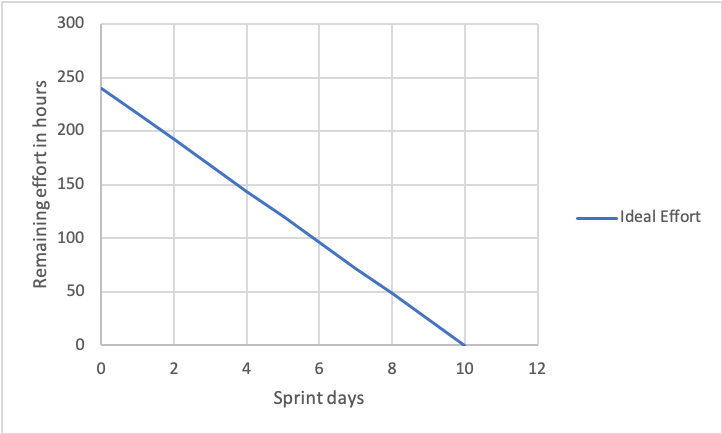
\includegraphics[width=0.6\textwidth]{images/burndown}
    \caption{Example sprint burn down chart}
\end{figure}

\subsubsection{Sprint Retrospective}
At the end of each sprint we will gather together and meet to discuss what will be needed in further sprints. The sprints wont have specific due dates
as the team would be able to communicates the status of their tasks.
\subsubsection{Individual Status Reports}
We will report to each other and communicate regularly about the updates on the project. We will note important points which will need to be discussed prior to deadlines.
\subsubsection{Engineering Notebooks}
The engineering notebook should be updated whenever ideas related to the project arise. Hopefully,
there would be a few updates between each meeting that we have regarding large changes to the project.


\subsection{Closeout Materials}
The following materials, in addition to major documentation deliverables, will be provided to the customer upon project closeout. Remove this paragraph from your draft, but leave the heading.

\subsubsection{System Prototype}
The Final System Prototype will have an android application that is well tested and properly functional. 
The Prototype shall be demonstrated to relevant stakeholders before the end of Senior Design 2. The team will 
be meeting with the project supervisor and customer on several occasions for Prototype Acceptance Test. This 
will help our team to ensure that we are moving in the right direction. There will be no demonstrations off-site 
therefore, no need for Field Acceptance Test.
\subsubsection{Project Poster}
The poster of our project will include our applications vision, mission and guidelines for installing 
the application. The Dimension of the poster approximately 20-30 inches wide and 30-40 inches tall. The poster 
will be delivered one day before the final presentation day of Senior Design 2.
\subsubsection{Web Page}
Web Page will contain the basic information of your project. This web page will help the readers learn more about 
the application and the team behind the application. The web page will consist of the team's vision, mission, 
background and introduction to the team members.
\subsubsection{Demo Video}
The Demo video will show the viewers how to install and use the software. 
It will inform the users about the major features of the application. The video will be 3-6 minutes long.
\subsubsection{Source Code}
The source code will be pushed to github repository periodically. The source code will only be available 
for team members until the project is complete. After the completion of project, the source code will be 
available to the sponsors of the project, and decision of making code available to public will be decided later.
\subsubsection{Source Code Documentation}
We will present our documentation in html format, with documentation for each function or parts of
the code.
\subsubsection{Installation Scripts}
The app will be available in app store so it will be very use to download and install.
\subsubsection{User Manual}
This app will be user friendly and very easy to use. The app will have short introduction video explaining 
about its features and how this app works so it will easy for everyone to use this app.